\documentclass[usenames,dvipsnames,handout,9pt]{beamer}
\usetheme[block=fill]{ru}           % Use ru theme

\usepackage{xpatch}
\usepackage{listings}
\usepackage{realboxes}

\definecolor{mygray}{rgb}{0.9,0.9,0.9}
\lstset{%
basicstyle=\ttfamily,
breaklines = true,
backgroundcolor=\color{mygray},
}

\makeatletter
\xpretocmd\lstinline{\Colorbox{mygray}\bgroup\appto\lst@DeInit{\egroup}}{}{}
\makeatother

\title{Advance Use of Git}

\author[Viguier]
{Beno\^{i}t Viguier}

\date[Short Occasion]{\vspace{0.5cm}DS-Lunch Talk,\\Nijmegen, March 12, 2019}

\begin{document}

% -------------------------------------------------------------

% -------------------------------------------------------------
\begin{frame}
  \titlepage
\end{frame}

% -------------------------------------------------------------

% -------------------------------------------------------------
\begin{frame}{Disclaimer}
\begin{center}
  \alert{\Large{\textbf{If you don't line Command Line Interface...\\This talk is not for you.}}}
\end{center}
\end{frame}

\begin{frame}{Minimal Git Commands}
  \begin{itemize}
    \item \lstinline|git clone git@gitlab.science.ru.nl:user/repo|
    \item \lstinline|git status|
    \item \lstinline|git add <directory/files>|
    \item \lstinline|git commit|
    \item \lstinline|git push|
    \item \lstinline|git pull|
  \end{itemize}
\end{frame}



%%%%%%%%%%%%%%%%%%%%%%%%%%%%%%%%%%%%%%%%%%%%%%%%%%%%%%%
%
%           Git Status
%           Git Log
%
%%%%%%%%%%%%%%%%%%%%%%%%%%%%%%%%%%%%%%%%%%%%%%%%%%%%%%%
\begin{frame}{Git Status}
\begin{itemize}
  \item \lstinline|git status|
  \item \lstinline|git log|
\end{itemize}

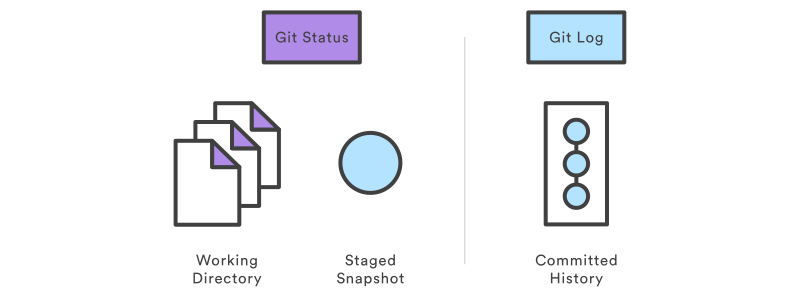
\includegraphics[width=0.8\textwidth]{img/inspecting/01.png}
\end{frame}


\begin{frame}{Shortcuts}
\begin{itemize}
  \item \lstinline|git add -A| \hspace{1cm}(\lstinline|-A| as All)\\
  \emph{Add all the updated/untracked files.}
  \item \lstinline|git add -u| \hspace{1cm}(\lstinline|-u| as update)\\
  \emph{Add all the updated files but do not add the untracked ones.}
  % \item \lstinline|git commit -a|\\
  % \emph{Equivalent to:} \lstinline|git add -u ; git commit|
  \item \lstinline|git commit -m "commit message"|
\end{itemize}
\end{frame}



\section{branches}

%%%%%%%%%%%%%%%%%%%%%%%%%%%%%%%%%%%%%%%%%%%%%%%%%%%%%%%
%
%          Branches
%
%%%%%%%%%%%%%%%%%%%%%%%%%%%%%%%%%%%%%%%%%%%%%%%%%%%%%%%
\begin{frame}{Branches}
\begin{itemize}
  \item Develop features without breaking master.\\
  $\implies$ the master branch always compiles! {\color{OliveGreen}\checkmark}
  \item Develop multiple features at the same time.

\end{itemize}
\vspace{0.5cm}
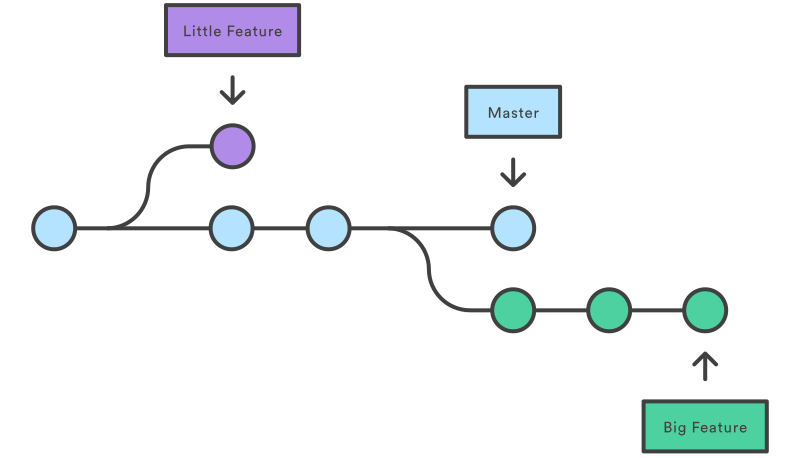
\includegraphics[width=0.8\textwidth]{img/branches/01.png}
\end{frame}

\begin{frame}{Branches}
  \vspace{-0.45cm}
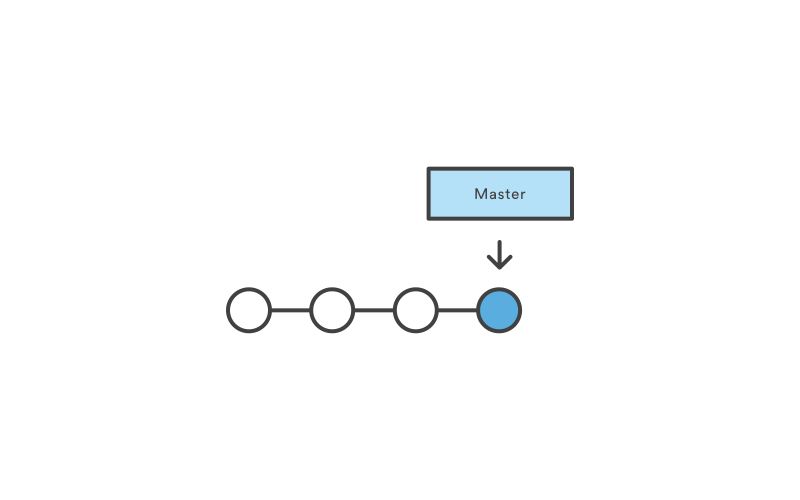
\includegraphics[width=0.8\textwidth]{img/branches/02.png}
\end{frame}

\begin{frame}{Branches}
  \begin{itemize}
    \item Create a branch \lstinline|git branch Future-plans|
    \item Switch to that branch \lstinline|git checkout Future-plans|
  \end{itemize}
\vspace{-1cm}
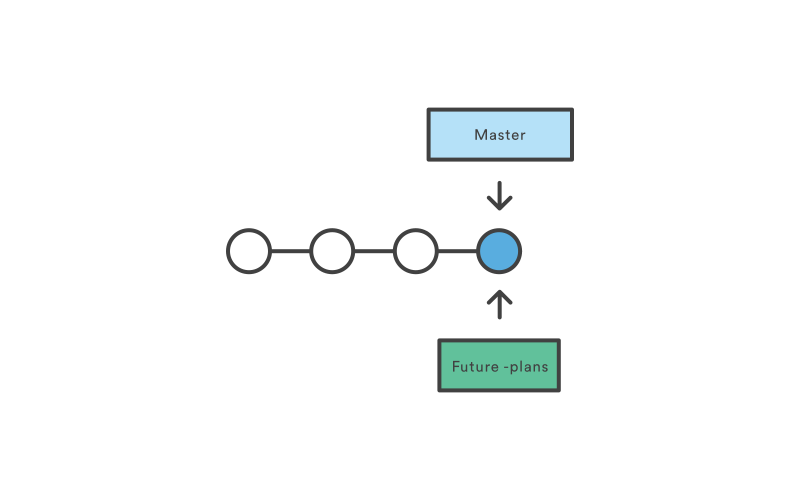
\includegraphics[width=0.8\textwidth]{img/branches/03.png}
\vspace{-1cm}

These two can be done in one step: \lstinline|git checkout -b Future-plans|
\end{frame}

\begin{frame}{Branches}
Work (modify, commits\ldots) on the \texttt{Future-plans}.\\
In the mean time, the \texttt{Master} branch continue forward (other commits\ldots)
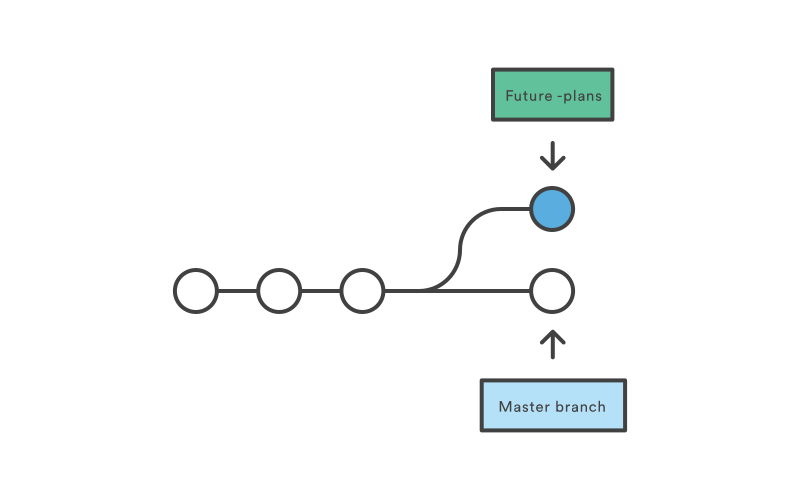
\includegraphics[width=0.8\textwidth]{img/branches/04.png}
\end{frame}


\begin{frame}{Branches}
If nothing was done on \texttt{Master} while you were working on \texttt{Future-plans} you can directly merge:
\begin{enumerate}
  \item Switch to the master branch: \lstinline|git checkout master|
  \item Merge: \lstinline|git merge Future-plans|
\end{enumerate}
\vspace{-1cm}
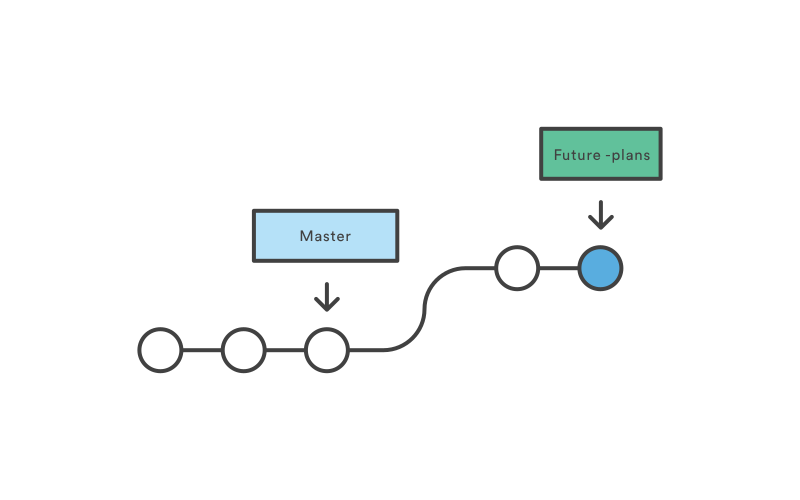
\includegraphics[width=0.8\textwidth]{img/branches/05.png}
\end{frame}

\begin{frame}{Branches}
\vspace{0.2cm}
If nothing was done on \texttt{Master} while you were working on \texttt{Future-plans} you can directly merge:
\begin{enumerate}
  \item Switch to the master branch: \lstinline|git checkout master|
  \item Merge: \lstinline|git merge Future-plans|
\end{enumerate}
\vspace{-0.8cm}
\hspace{0.07cm}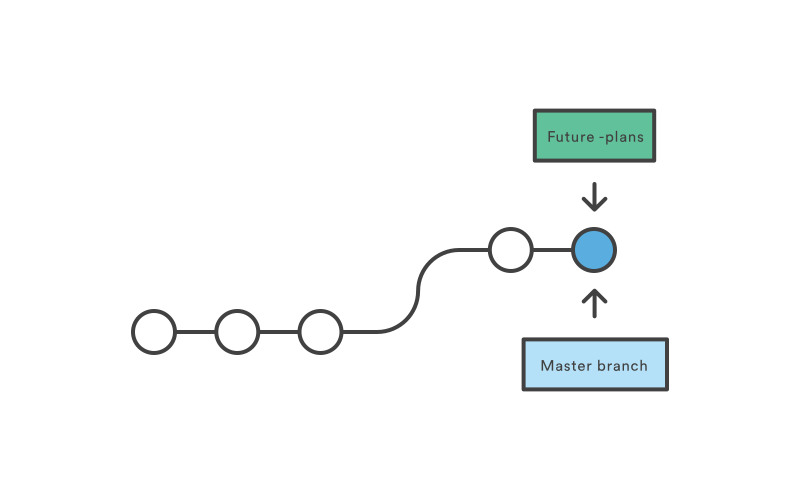
\includegraphics[width=0.8\textwidth]{img/branches/06.png}
\end{frame}

\begin{frame}{Branches}
  \centering
  To delete a branch, you do \lstinline|git branch -D <branch-name>|\\
  \lstinline|-D| as Delete\\
  (Not possible while you are on that branch)
\end{frame}



%%%%%%%%%%%%%%%%%%%%%%%%%%%%%%%%%%%%%%%%%%%%%%%%%%%%%%%
%
%          Merging
%
%%%%%%%%%%%%%%%%%%%%%%%%%%%%%%%%%%%%%%%%%%%%%%%%%%%%%%%

\begin{frame}{Merging}
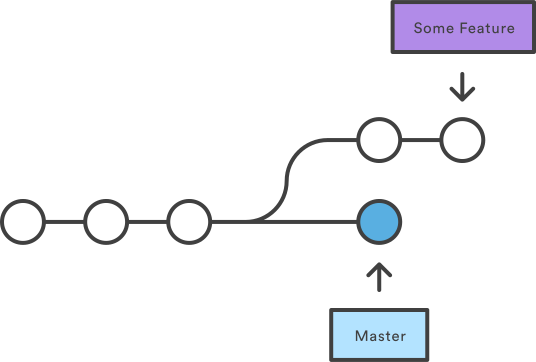
\includegraphics[width=0.608\textwidth]{img/merge/08.png}
\end{frame}

\begin{frame}{Merging}
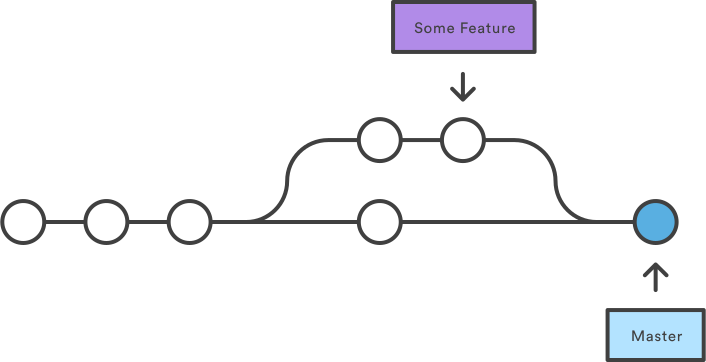
\includegraphics[width=0.8\textwidth]{img/merge/09.png}
\end{frame}



















\begin{frame}[fragile]{bonus}
  In your \texttt{~\char`\\.bashrc} or \texttt{~\char`\\.zshrc}:

  \texttt{alias gtree='git log --oneline --decorate --all --graph'}
\end{frame}
% commit
% branch
% checkout
% cherry-pick
% reset
% revert
% rebase
% merge
% cherry-pick



% <<<<<<< HEAD
% =======
% >>>>>>> new_branch_to_merge_later



\end{document}
